%******************************************************************************%
%                                                                              %
%                   Machine_Learning_01.tex                                    %
%                   Made by: lganti, ikourkji                                  %
%                                                                              %
%******************************************************************************%

\documentclass{42-en}
%\usepackage[document]{ragged2e}
\usepackage{pythonhighlight}
%\usepackage{listings}


\begin{document}

\title{Introduction to Machine Learning}
\subtitle{Numpy, Pandas, Matplotlib: Basic Exercises}

\member {Jeson}{junzhen@42.us.org}
\member {}{Jesonleejunzhen.com}

\summary 
{
Learn about the essential Python libraries for machine learning
}

\maketitle

\tableofcontents

%Initialisation des headers d'exercices

\newpage

\bigskip

\centerline{
\includegraphics[width=150mm]{images/dontpanic.png}}

\centerline{\texttt{Eat, Sleep, Code, Repeat.}}

%******************************************************************************%
%                                                                              %
%                                 Don't Panic                                  %
%                                                                              %
%******************************************************************************%
\chapter{Intro to NumPy}

\centerline{
\includegraphics[width=150mm]{images/too_much_linkedin.png}}

\raggedright{
Before we dive into learning about ‘machine learning’, let’s take a look at some of the essential programming skills needed to build a machine learning project using Python. 
}\linebreak

\raggedright{
Some of the most commonly used python libraries are Numpy, Pandas, and Matplotlib.
}\linebreak

\raggedright{
These powerful libraries can be used to pre-process, analyze, and visualize data before we even begin building a machine learning model.
}\linebreak

\raggedright{
So let’s not waste time and dive straight into it! Let’s start off with downloading the libraries by doing this:
}

\vspace{1em}
\begin{lstlisting}
pip3 install numpy
pip3 install pandas
pip3 install matplotlib
\end{lstlisting}

\vspace{1em}

You may need to add the ‘--user’ flag in order to add the libraries to your home directory, which won’t require any special privileges.\linebreak \linebreak

\chapter{Numpy}

\vspace{2em}


\includegraphics[width=80mm, height=30mm]{images/numpy.jpeg}

\vspace{1em}

\raggedright{Numpy is a math library for python. It enables us to do computation efficiently and effectively. Numpy has many amazing capabilities such as the ability to manipulate large arrays and matrices of numeric data.\linebreak

To use the NumPy module, we need to import it using:\linebreak

\begin{lstlisting}
    import numpy as np
\end{lstlisting}

\vspace{1em}
Take a look at \href{https://s3.amazonaws.com/assets.datacamp.com/blog_assets/Numpy_Python_Cheat_Sheet.pdf}{this Numpy cheat sheet by DataCamp} to get an overall understanding.}

\startexercices


% % % % % % % % % % EX00 % % % % % % % % % % % % 

\chapter{Exercise 00: Creating a numpy array using arange}
\exfiles{00\_numpy\_array.py}
\extitle{Creating a numpy array using arange}
\turnindir{numpy}
\extopics{Numpy Array}
\makeheaderfiles

Create a Numpy array using arange. A NumPy array is a grid of values. They are similar to lists, except that every element of an array must be the same type. Write a program that will print the following output.

\vspace{1em}
Desired output:
\vspace{1em}
\begin{42console}
#> [0 1 2 3 4 5 6 7 8 9]
\end{42console}
\vspace{1em}
\textbf{Okay, but why do I have to use an np array rather than a regular array?}\linebreak

Numpy arrays are better in terms of faster computation and ease of manipulation.\linebreak

More information: \href{ https://stackoverflow.com/questions/993984/what-are-the-advantages-of-numpy-over-regular-python-lists/994010#994010}{ https://stackoverflow.com/questions/993984/what-are-the-advantages-of-numpy-over-regular-python-lists/994010#994010 }

\nextexercice
\newpage

% % % % % % % % % % EX01 % % % % % % % % % % % % 

\chapter{Exercise 01: Extract elements from an array}
\exfiles{01\_operator.py}
\extitle{Extract elements from an array}
\turnindir{numpy}
\extopics{Operator}
\makeheaderfiles

\vspace{1em}
Declare and initialize an array as done below: \linebreak
\begin{lstlisting}
    arr = np.array([0, 1, 2, 3, 4, 5, 6, 7, 8, 9])
\end{lstlisting}
\vspace{1em}
Then, extract all odd numbers from arr to achieve the desired output.\linebreak
Desired output:
\vspace{1em}
\begin{42console}
#> [1 3 5 7 9]
\end{42console}
\nextexercice
\newpage


% % % % % % % % % % EX02 % % % % % % % % % % % % 


\chapter{Exercise 02: Converting a one-dimensional array to two-dimensional}

\exfiles{02\_dimensions.py}
\extitle{Converting a one-dimensional array to two-dimensional}
\turnindir{numpy}
\extopics{Arrange, Reshape}
\makeheaderfiles
\vspace{1em}
Convert a 1D array to a 2D array with 2 rows using arange 
\vspace{0.8em}

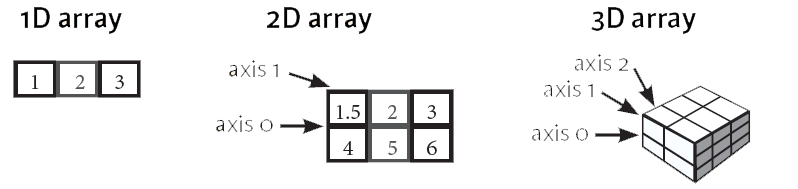
\includegraphics[width=150mm]{images/content_arrays-axes.png}

\vspace{0.8em}

Declare and initialize an array as done below
\vspace{1em}

\begin{lstlisting}
   np.arange(10)
\end{lstlisting}

\vspace{1em}

Try recreating this output:\linebreak
\begin{42console}
#>[[0 1 2 3 4]
   [5 6 7 8 9]]
\end{42console}

\nextexercice
\newpage

% % % % % % % % % % EX03 % % % % % % % % % % % % 


\chapter{Exercise 03:  Inspecting a numpy array}
\exfiles{03\_dimensions.py}
\extitle{Inspecting a numpy array}
\turnindir{numpy}
\extopics{Python Objects}
\makeheaderfiles
\vspace{1em}
Create a 2d array with 3 rows and 4 columns
\vspace{1em}

\begin{lstlisting}
   myList = [[1, 2, 3, 4],[3, 4, 5, 6], [5, 6, 7, 8]]
\end{lstlisting}

\vspace{1em}
Inspect its shape, datatype, size, number dimensions 
\nextexercice
\newpage

% % % % % % % % % % EX04 % % % % % % % % % % % % 


\chapter{Exercise 04:  Stack them (arrays) up!}
\exfiles{04\_stack.py}
\extitle{Stack them (arrays) up!}
\turnindir{numpy}
\extopics{2D array}
\makeheaderfiles
\vspace{1em}
Stack the arrays a and b vertically
\vspace{1em}

\begin{lstlisting}
    a = np.arange(10).reshape(2,-1)
    b = np.repeat(1, 10).reshape(2,-1)
\end{lstlisting}

\vspace{1em}
Try creating this output:\linebreak
\begin{42console}
#> [[0 1 2 3 4]
    [5 6 7 8 9]
    [1 1 1 1 1]
    [1 1 1 1 1]]
\end{42console}
\nextexercice
\newpage

% % % % % % % % % % EX05 % % % % % % % % % % % % 


\chapter{Exercise 05:  Replacing missing value}
\exfiles{05\_replace.py}
\extitle{Replacing missing value}
\turnindir{numpy}
\extopics{isnan, isnif}
\makeheaderfiles
\vspace{1em}

\begin{lstlisting}
    myList = [[1, 2, 3, 4],[3, 4, 5, 6], [5, 6, 7, 8]]
    arr = np.array(myList, dtype='float')
    arr[1,1] = np.nan  # not a number
    arr[1,2] = np.inf  # infinite
    print(arr)
\end{lstlisting}

\vspace{1em}
Output:\linebreak
\begin{42console}
#> [[ 1.  2.  3.  4.]
    [ 3. -1. -1.  6.]
    [ 5.  6.  7.  8.]]
\end{42console}
\nextexercice
\newpage


% % % % % % % % % % EX06 % % % % % % % % % % % % 


\chapter{Exercise 06:  Drop all missing values from a numpy array}
\exfiles{06\_drop.py}
\extitle{Drop all missing values from a numpy array}
\turnindir{numpy}
\extopics{isnan}
\makeheaderfiles
\vspace{1em}

\begin{lstlisting}
     np.array([1,2,3,np.nan,5,6,7,np.nan])
\end{lstlisting}

\vspace{1em}
Output:\linebreak
\begin{42console}
[ 1.  2.  3.  5.  6.  7.]
\end{42console}
\nextexercice
\newpage

% % % % % % % % % % EX07 % % % % % % % % % % % % 


\chapter{Exercise 07:  Find duplicate records in a numpy array}
\exfiles{07\_duplicate.py}
\extitle{Find duplicate records in a numpy array}
\turnindir{numpy}
\extopics{np.unique}
\makeheaderfiles
\vspace{1em}
Stack the arrays a and b vertically
\vspace{1em}

\begin{lstlisting}
    np.random.seed(100)
    a = np.random.randint(0, 5, 10)
    print('Array: ', a)
\end{lstlisting}

\vspace{1em}

\textbf{Mark the unique position as false}
 
\vspace{1em}
 
Output:\linebreak
\begin{42console}
#> [False  True False  True False False  True  True  True  True]
\end{42console}

\chapter{Pandas}

\centerline{
\includegraphics[width=150mm]{images/panda.jpeg}}

Pandas is one of the most popular Python libraries for Data Science and Analytics. I like to say it’s the “SQL of Python.” Why? Because pandas helps you to manage two-dimensional data tables in Python. Of course, it has many more features, let’s explore the power of pandas in this tutorial.\\
To use pandas, we need to import it using:\\
\begin{lstlisting}
    import pandas as pd
\end{lstlisting}
Take a look at \href{https://s3.amazonaws.com/assets.datacamp.com/blog_assets/PandasPythonForDataScience.pdf}{this pandas cheat sheet by DataCamp} to get an overall understanding.

% % % % % % % % % % EX00 % % % % % % % % % % % % 

\chapter{Exercise 00: Series}
\exfiles{00\_series.py}
\turnindir{pandas}
\extitle{Series}
\extopics{Series}
\makeheaderfiles

Create a one-dimensional labeled array capable of holding any data type using a Series.\\

\begin{42console}
#> A    3
#> B    5
#> C    7
#> D    4
\end{42console}

\nextexercice
\newpage

% % % % % % % % % % EX01 % % % % % % % % % % % % 

\chapter{Exercise 01: DataFrame}
\exfiles{01\_data\_frame.py}
\extitle{DataFrame}
\turnindir{pandas}
\extopics{DataFrame}
\makeheaderfiles

\vspace{1em}
Create a two-dimensional labeled data structure with columns of potentially different types using a DataFrame. \linebreak
Example:\\
\begin{42console}
data = {'Country': ['Belgium', 'India', 'Brazil'],
'Capital': ['Brussels', 'New Delhi', 'Brasilia'],
'Population': [11190846, 1303171035, 207847528]}
\end{42console}
\linebreak
\begin{table}[!ht]
\centering
\begin{tabular}{|l|l|l|l|}
\hline
  & Country & Capital   & Population \\ \hline
1 & Belgium & Brussels  & 11190846   \\ \hline
2 & India   & New Delhi & 1303171035 \\ \hline
3 & Brazil  & Brasilia  & 207847     \\ \hline
\end{tabular}
\end{table}
\linebreak
Now take this data:\\
\begin{42console}
data = {'animal': ['cat', 'cat', 'snake', 'dog', 'dog', 'cat', 'snake', 'cat', 'dog', 'dog'],
    'age': [2.5, 3, 0.5, np.nan, 5, 2, 4.5, np.nan, 7, 3],
    'visits': [1, 3, 2, 3, 2, 3, 1, 1, 2, 1],
    'priority': ['yes', 'yes', 'no', 'yes', 'no', 'no', 'no', 'yes', 'no', 'no']}
    
labels = ['a', 'b', 'c', 'd', 'e', 'f', 'g', 'h', 'i', 'j']
\end{42console}
Using the dictionary above, answer the next 6 questions.
\nextexercice
\newpage


% % % % % % % % % % EX02 % % % % % % % % % % % % 


\chapter{Exercise 02: Display summary}

\exfiles{02\_display.py}
\extitle{Display summary}
\turnindir{pandas}
\extopics{info(), describe()}
\makeheaderfiles
Display a summary of the basic information about this DataFrame and its data.\\
\nextexercice
\newpage

% % % % % % % % % % EX03 % % % % % % % % % % % % 


\chapter{Exercise 03:  Displaying rows}
\exfiles{03\_rows.py}
\extitle{Displaying rows}
\turnindir{pandas}
\extopics{iloc}
\makeheaderfiles

Return the first 3 rows of the DataFrame df.

\nextexercice
\newpage

% % % % % % % % % % EX04 % % % % % % % % % % % % 


\chapter{Exercise 04:  Retrieving data}
\exfiles{04\_retrieve.py}
\extitle{Retrieving data}
\turnindir{pandas}
\extopics{.between()}
\makeheaderfiles
Select the rows the age is between 2 and 4 (inclusive).\\
\nextexercice
\newpage

% % % % % % % % % % EX05 % % % % % % % % % % % % 


\chapter{Exercise 05: Adding and dropping data}
\exfiles{05\_adding\_dropping.py}
\extitle{Adding and dropping data}
\turnindir{pandas}
\extopics{drop()}
\makeheaderfiles

Append a new row \texttt{'k'} to df with your choice of values for each column. Then delete that row to return the original DataFrame.\\

\nextexercice
\newpage


% % % % % % % % % % EX06 % % % % % % % % % % % % 


\chapter{Exercise 06: Calculate}
\exfiles{06\_calculate.py}
\extitle{Calculate}
\turnindir{pandas}
\extopics{group\_by()}
\makeheaderfiles
Calculate the mean age for each different animal in df.\\
\nextexercice
\newpage

% % % % % % % % % % EX07 % % % % % % % % % % % % 


\chapter{Exercise 07:  Sorting}
\exfiles{07\_sort.py}
\extitle{Sorting}
\turnindir{pandas}
\extopics{sort\_values()}
\makeheaderfiles
Sort df first by the values in the \texttt{'age'} in descending order, then by the values in the \texttt{'visit'} column in ascending order.\\

\chapter{Matplotlib}

Matplotlib is a python library used to create 2D graphs and plots. It has a module named pyplot which makes things easy for plotting by providing features to control line styles, font properties, formatting axes etc.\\

To use Matplotlib, we need to import it using:\\

\begin{lstlisting}
    import matplotlib.pyplot as plt
\end{lstlisting}

Take a look at \href{https://s3.amazonaws.com/assets.datacamp.com/blog_assets/Python_Matplotlib_Cheat_Sheet.pdf}{this matplotlib cheat sheet by DataCamp} to get an overall understanding.

\centerline{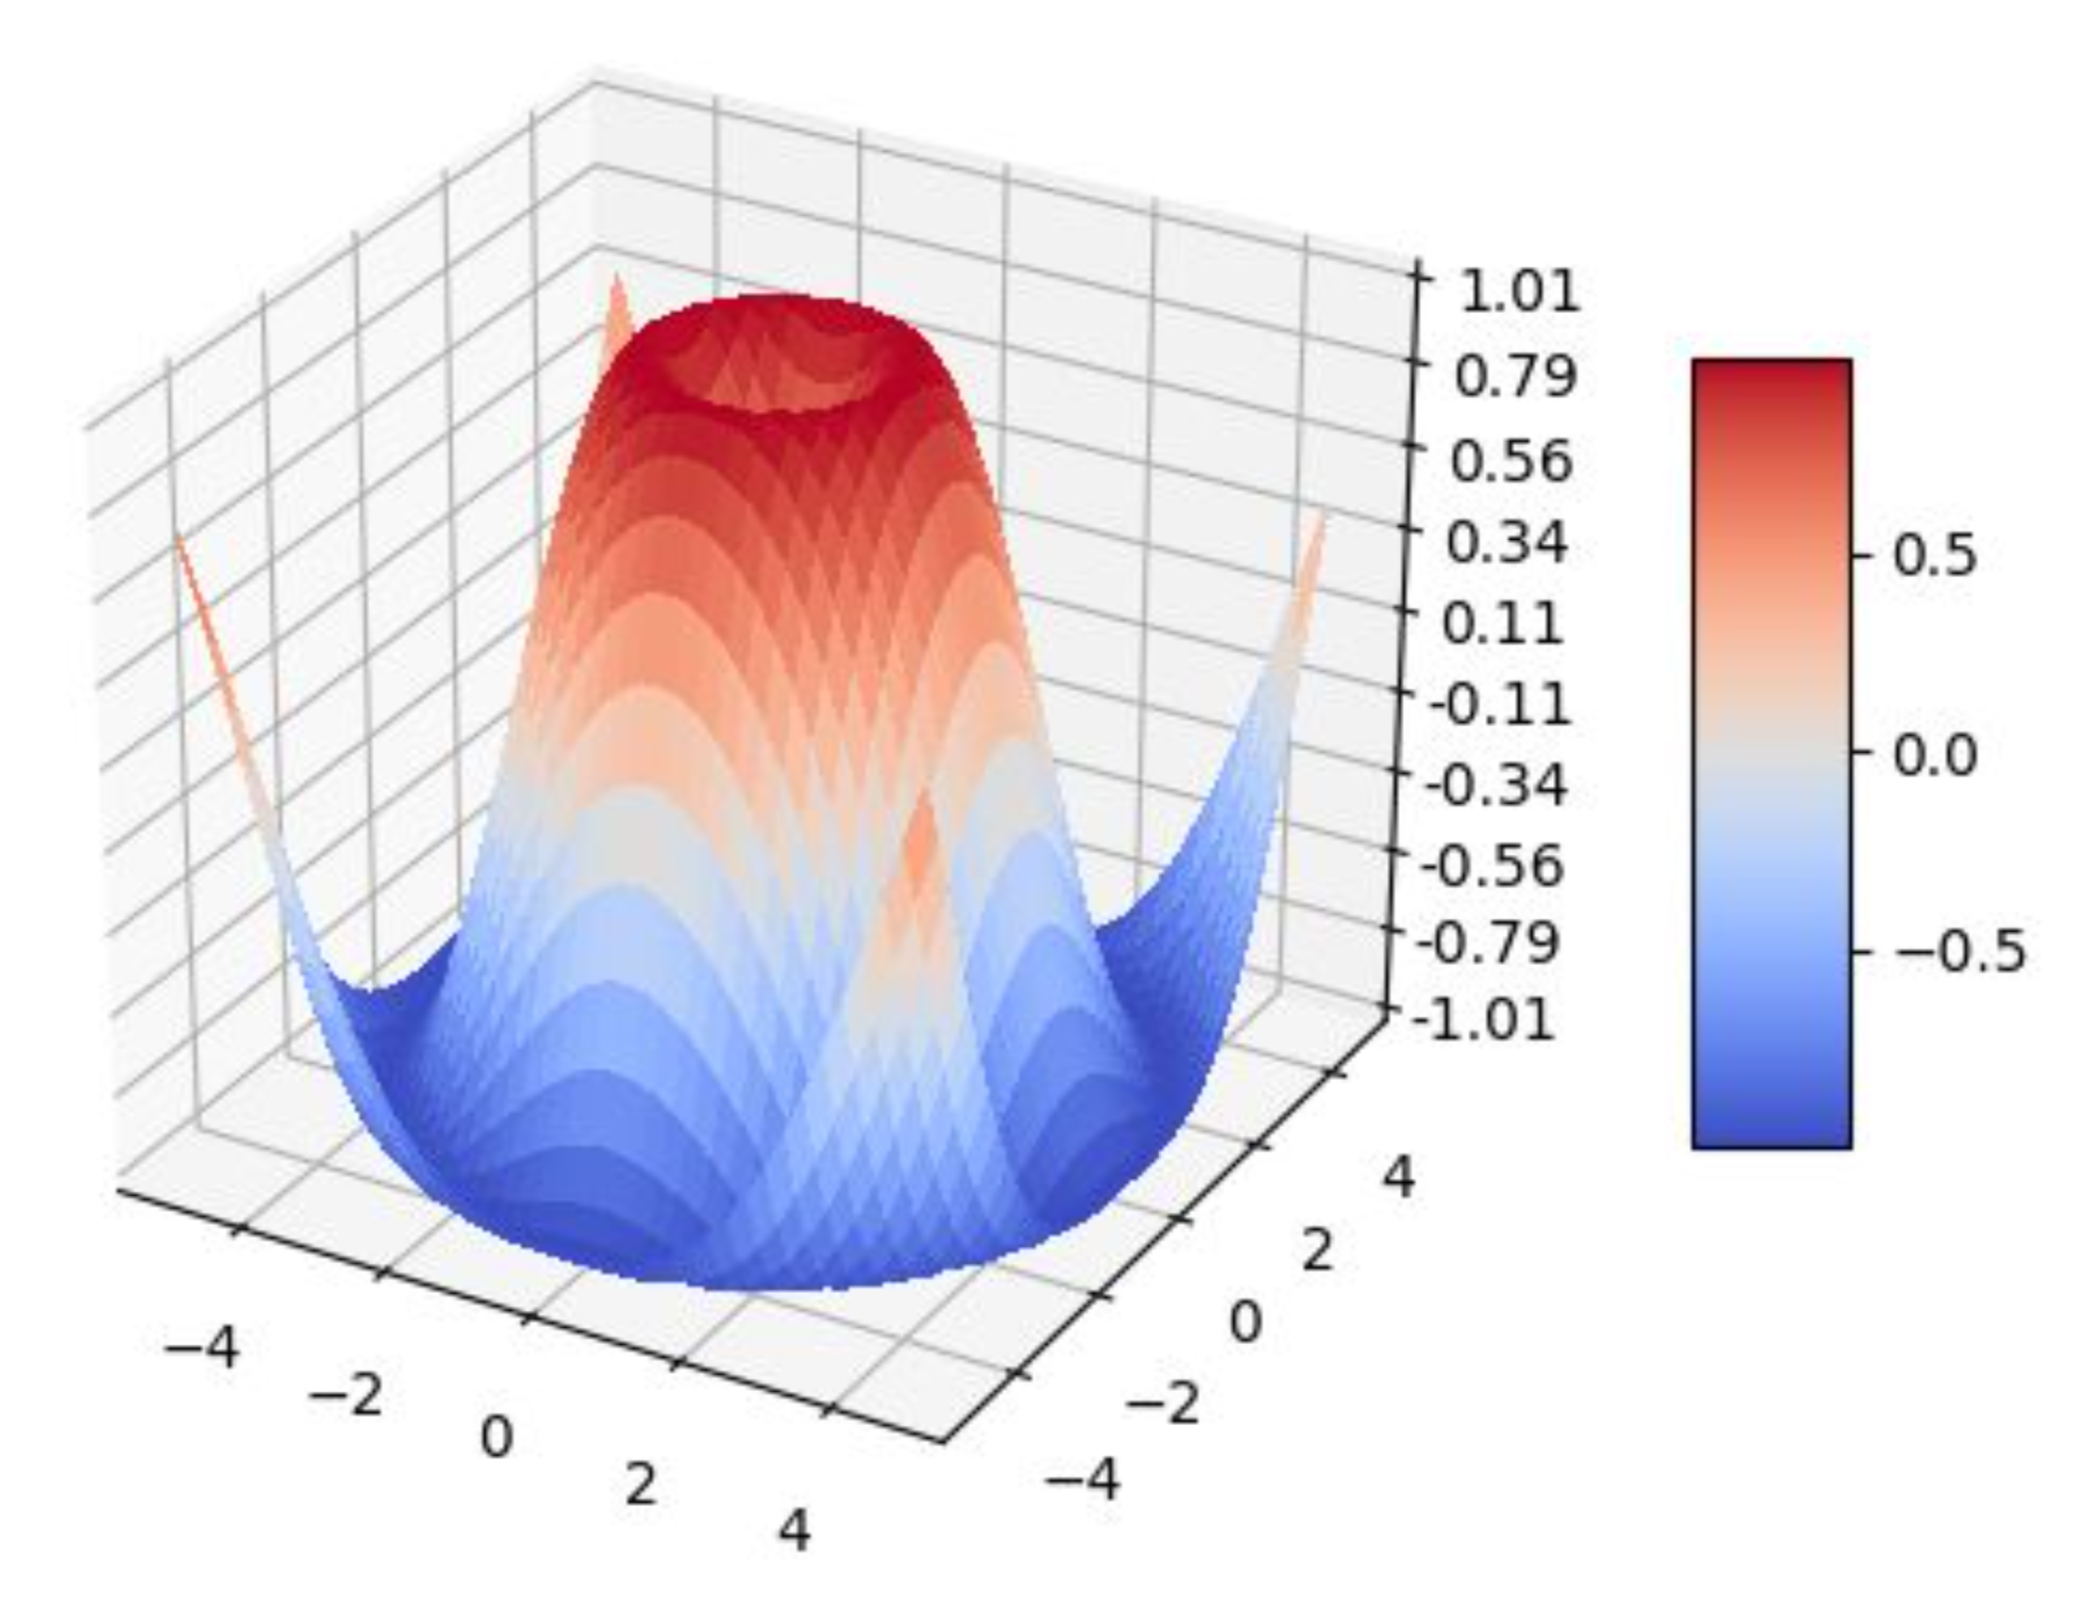
\includegraphics[width=150mm]{images/3d_graph.png}}

% % % % % % % % % % EX00 % % % % % % % % % % % % 

\chapter{Exercise 00: Linear graph}
\exfiles{00\_linear\_graph.py}
\turnindir{matplotlib}
\extitle{Linear graph}
\extopics{plotting}
\makeheaderfiles

Plot this linear graph using matplotlib.\\

\centerline{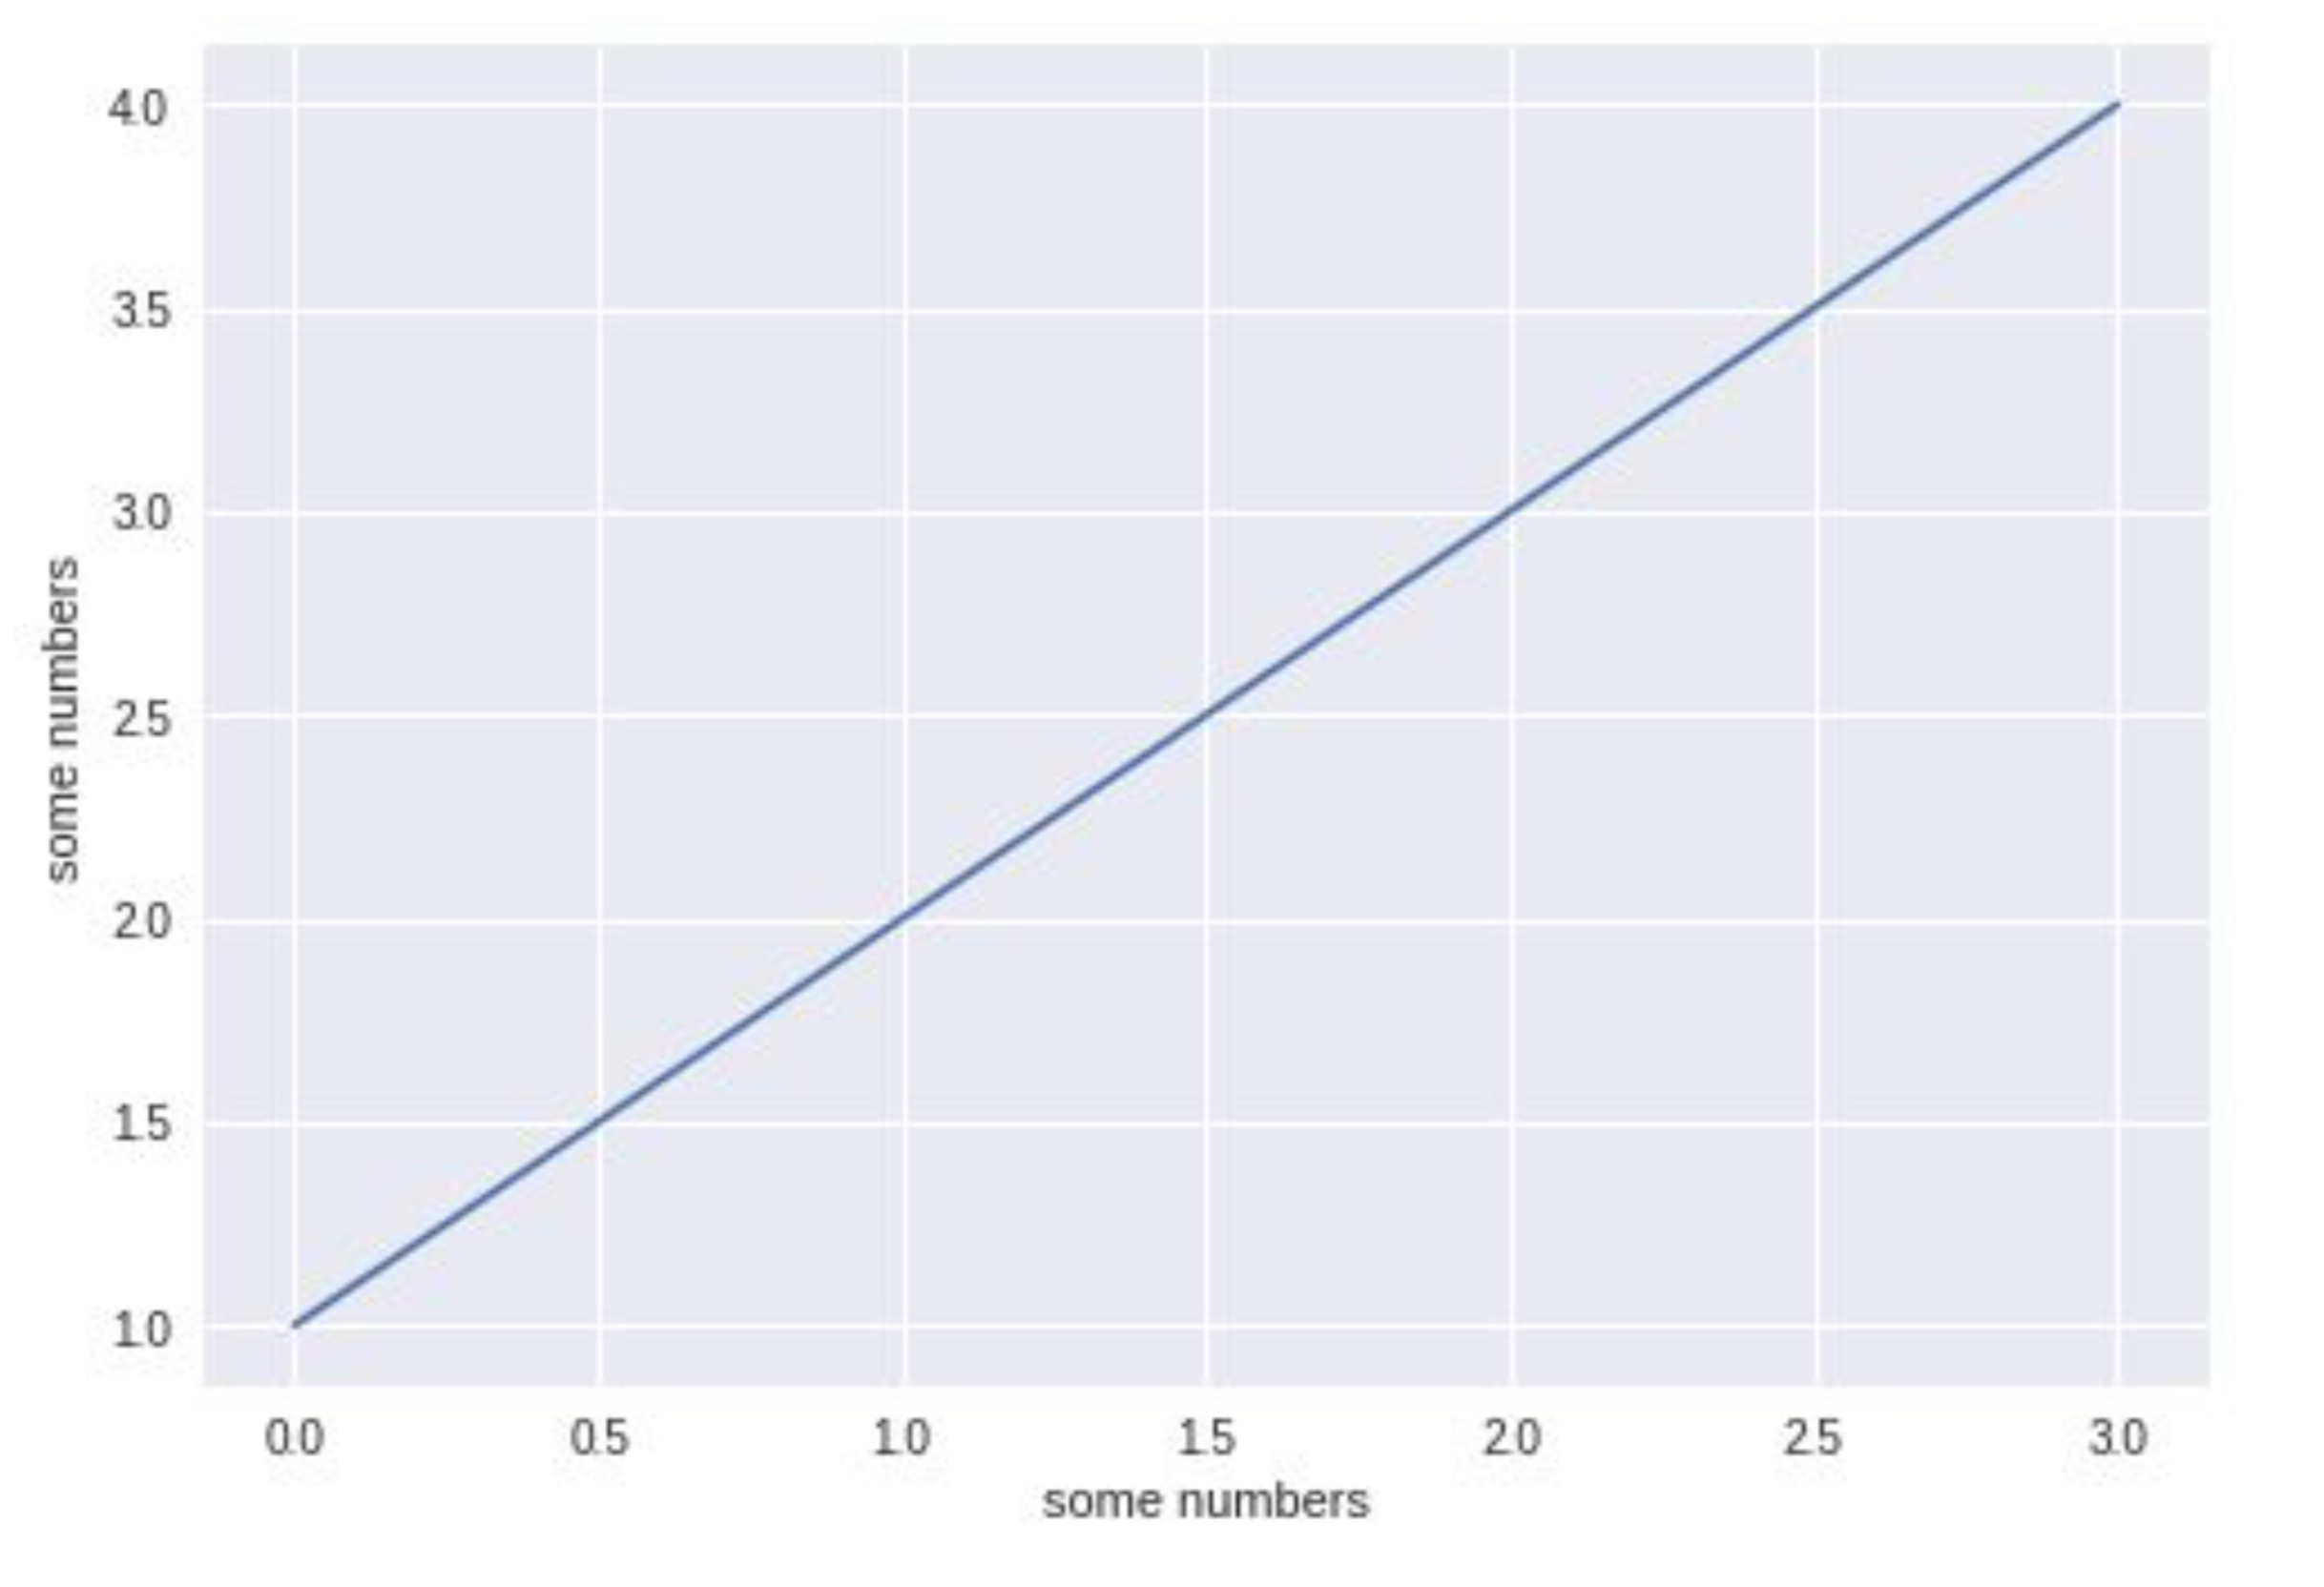
\includegraphics[width=150mm]{images/boring_line.png}}

\nextexercice
\newpage

% % % % % % % % % % EX01 % % % % % % % % % % % % 

\chapter{Exercise 01: Linear circle graph}
\exfiles{01\_linear\_circle.py}
\turnindir{matplotlib}
\extitle{Linear circle graph}
\extopics{plotting}
\makeheaderfiles

Plot this linear graph using matplotlib with this data:\\

\begin{lstlisting}
    import numpy as np
    x = np.arange(1,11)
    y = 2 * x + 5
\end{lstlisting}

\centerline{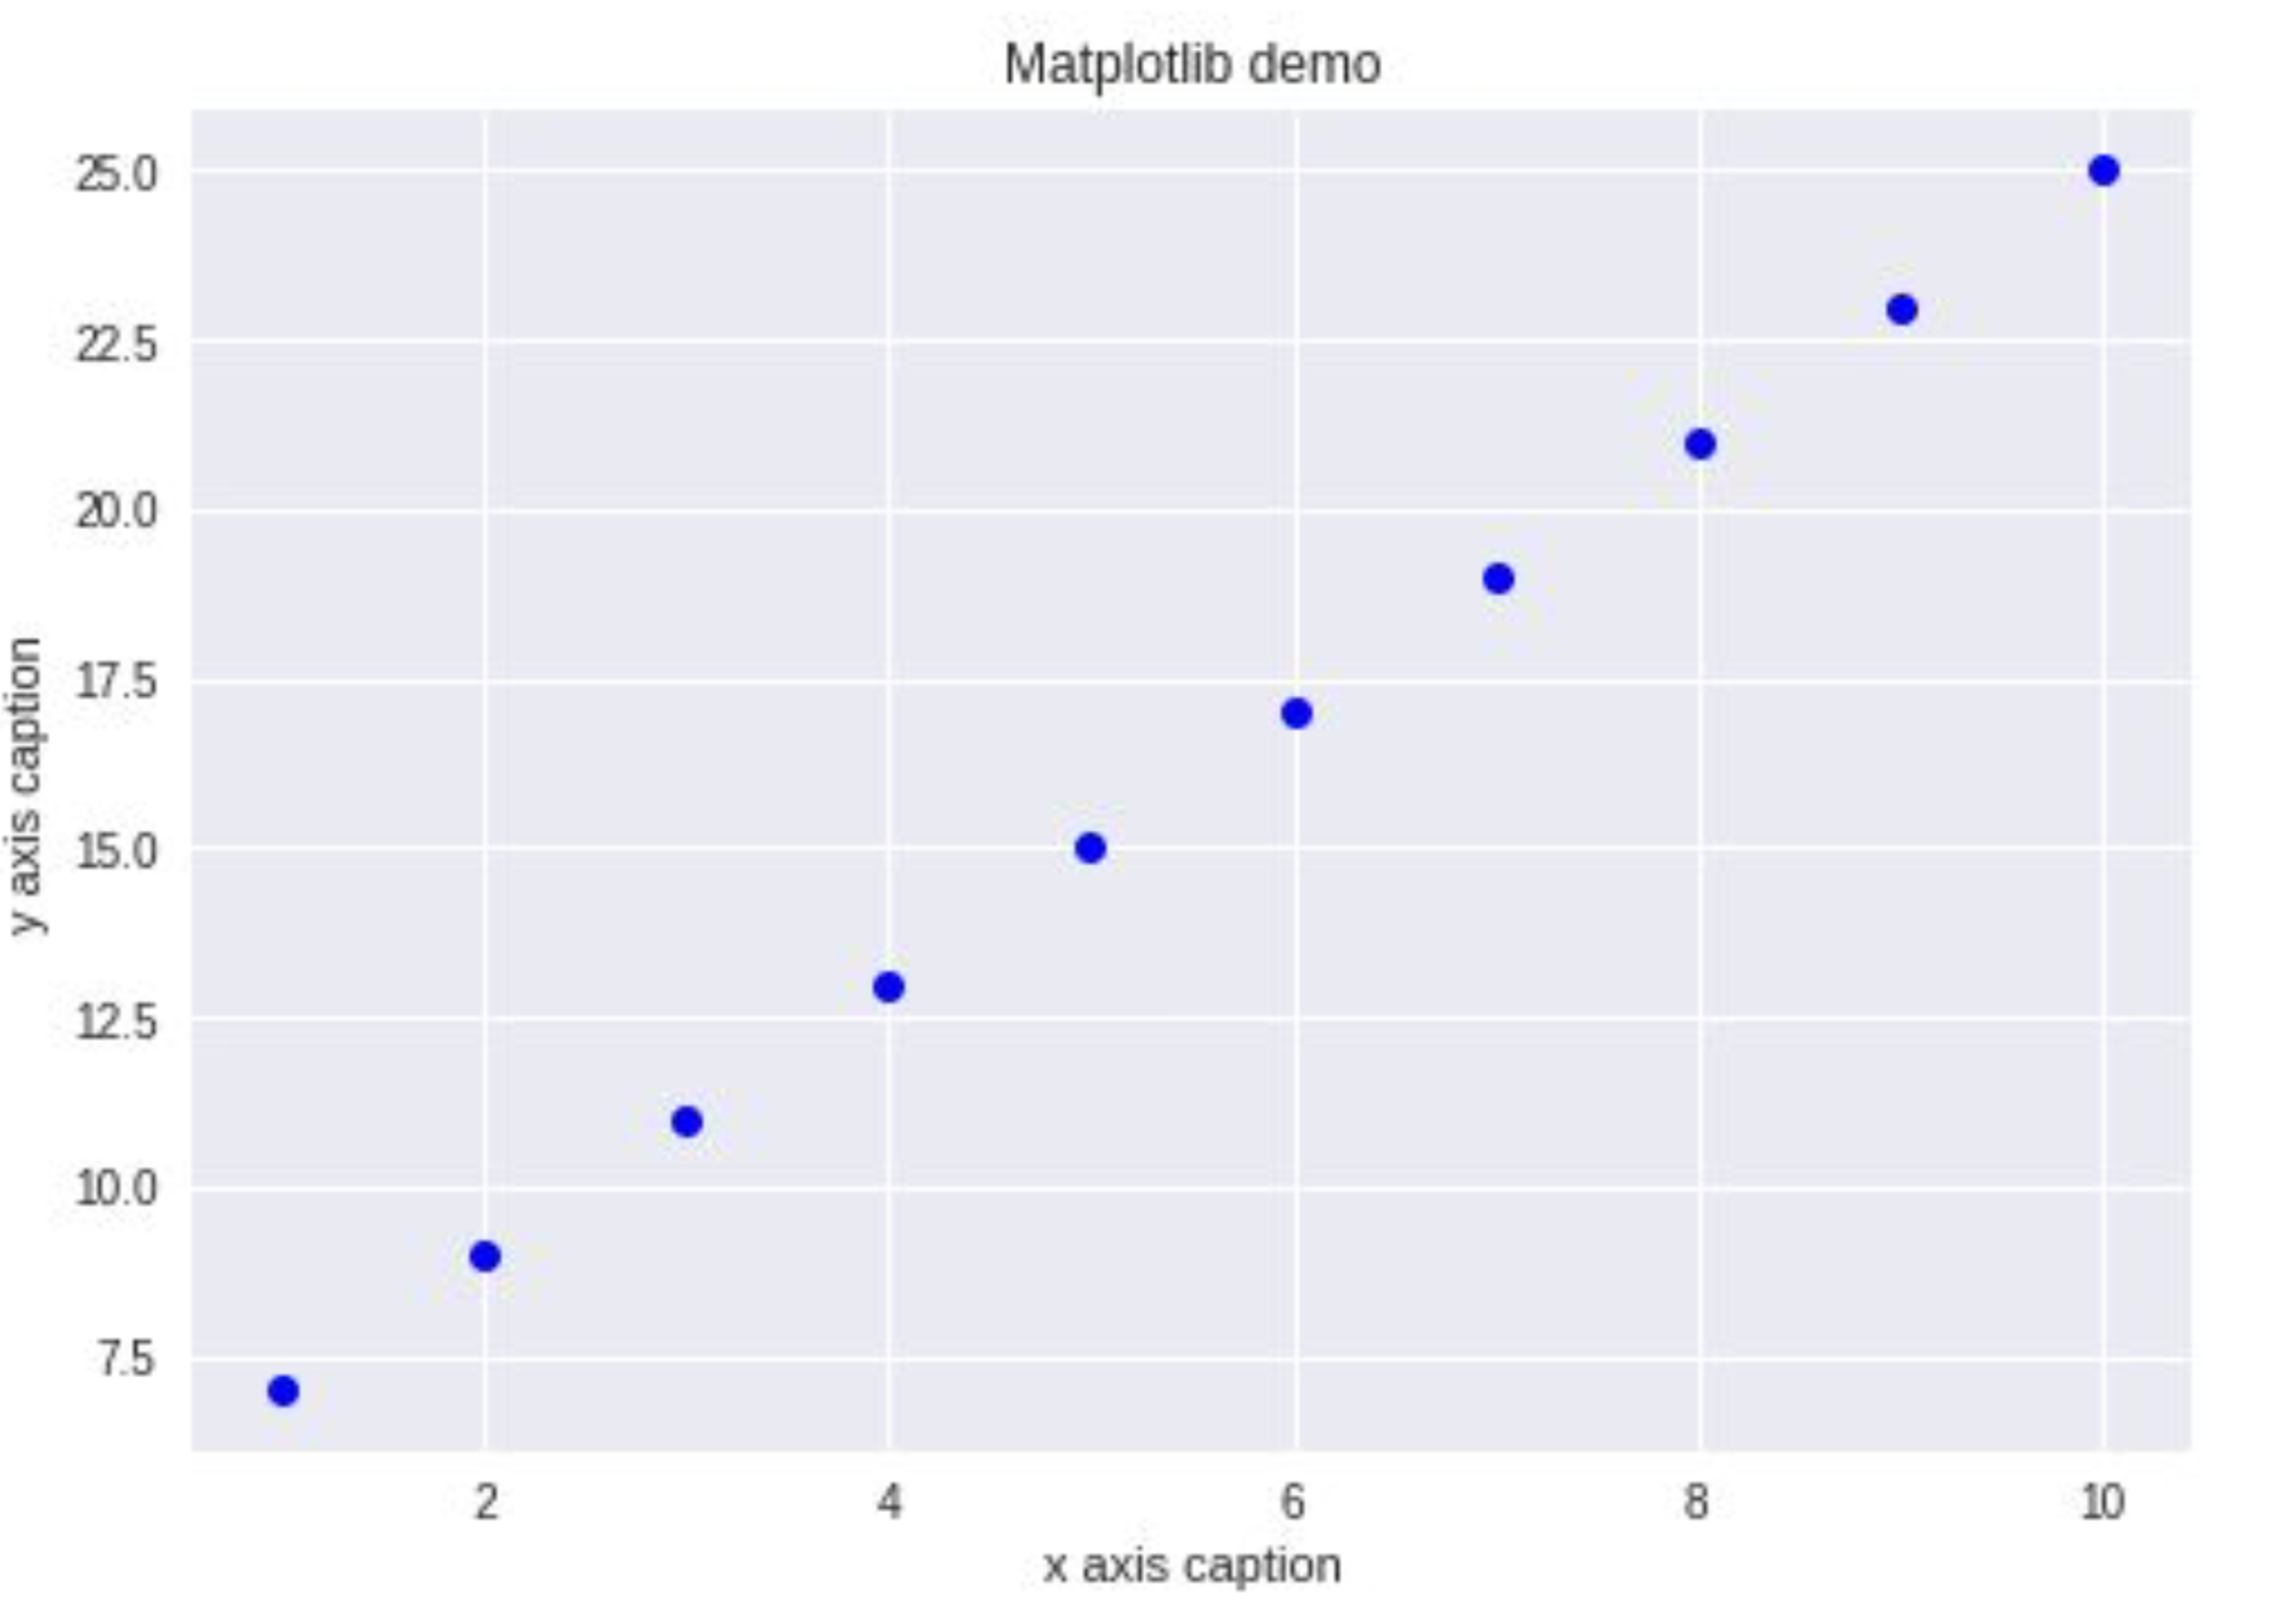
\includegraphics[width=125mm]{images/linear_pts.png}}

\nextexercice
\newpage


% % % % % % % % % % EX02 % % % % % % % % % % % % 


\chapter{Exercise 02: Bar graph}

\exfiles{02\_bar.py}
\turnindir{matplotlib}
\extitle{Bar graph}
\extopics{plotting}
\makeheaderfiles

Plot a bar graph with this data:\\

\begin{lstlisting}
    import matplotlib.pyplot as plt; plt.rcdefaults()
    import numpy as np
    import matplotlib.pyplot as plt
    
    objects = ('Python', 'C++', 'Java', 'Perl', 'Scala', 'Lisp')
    y_pos = np.arange(len(objects))
    performance = [10,8,6,4,2,1]
\end{lstlisting}

\centerline{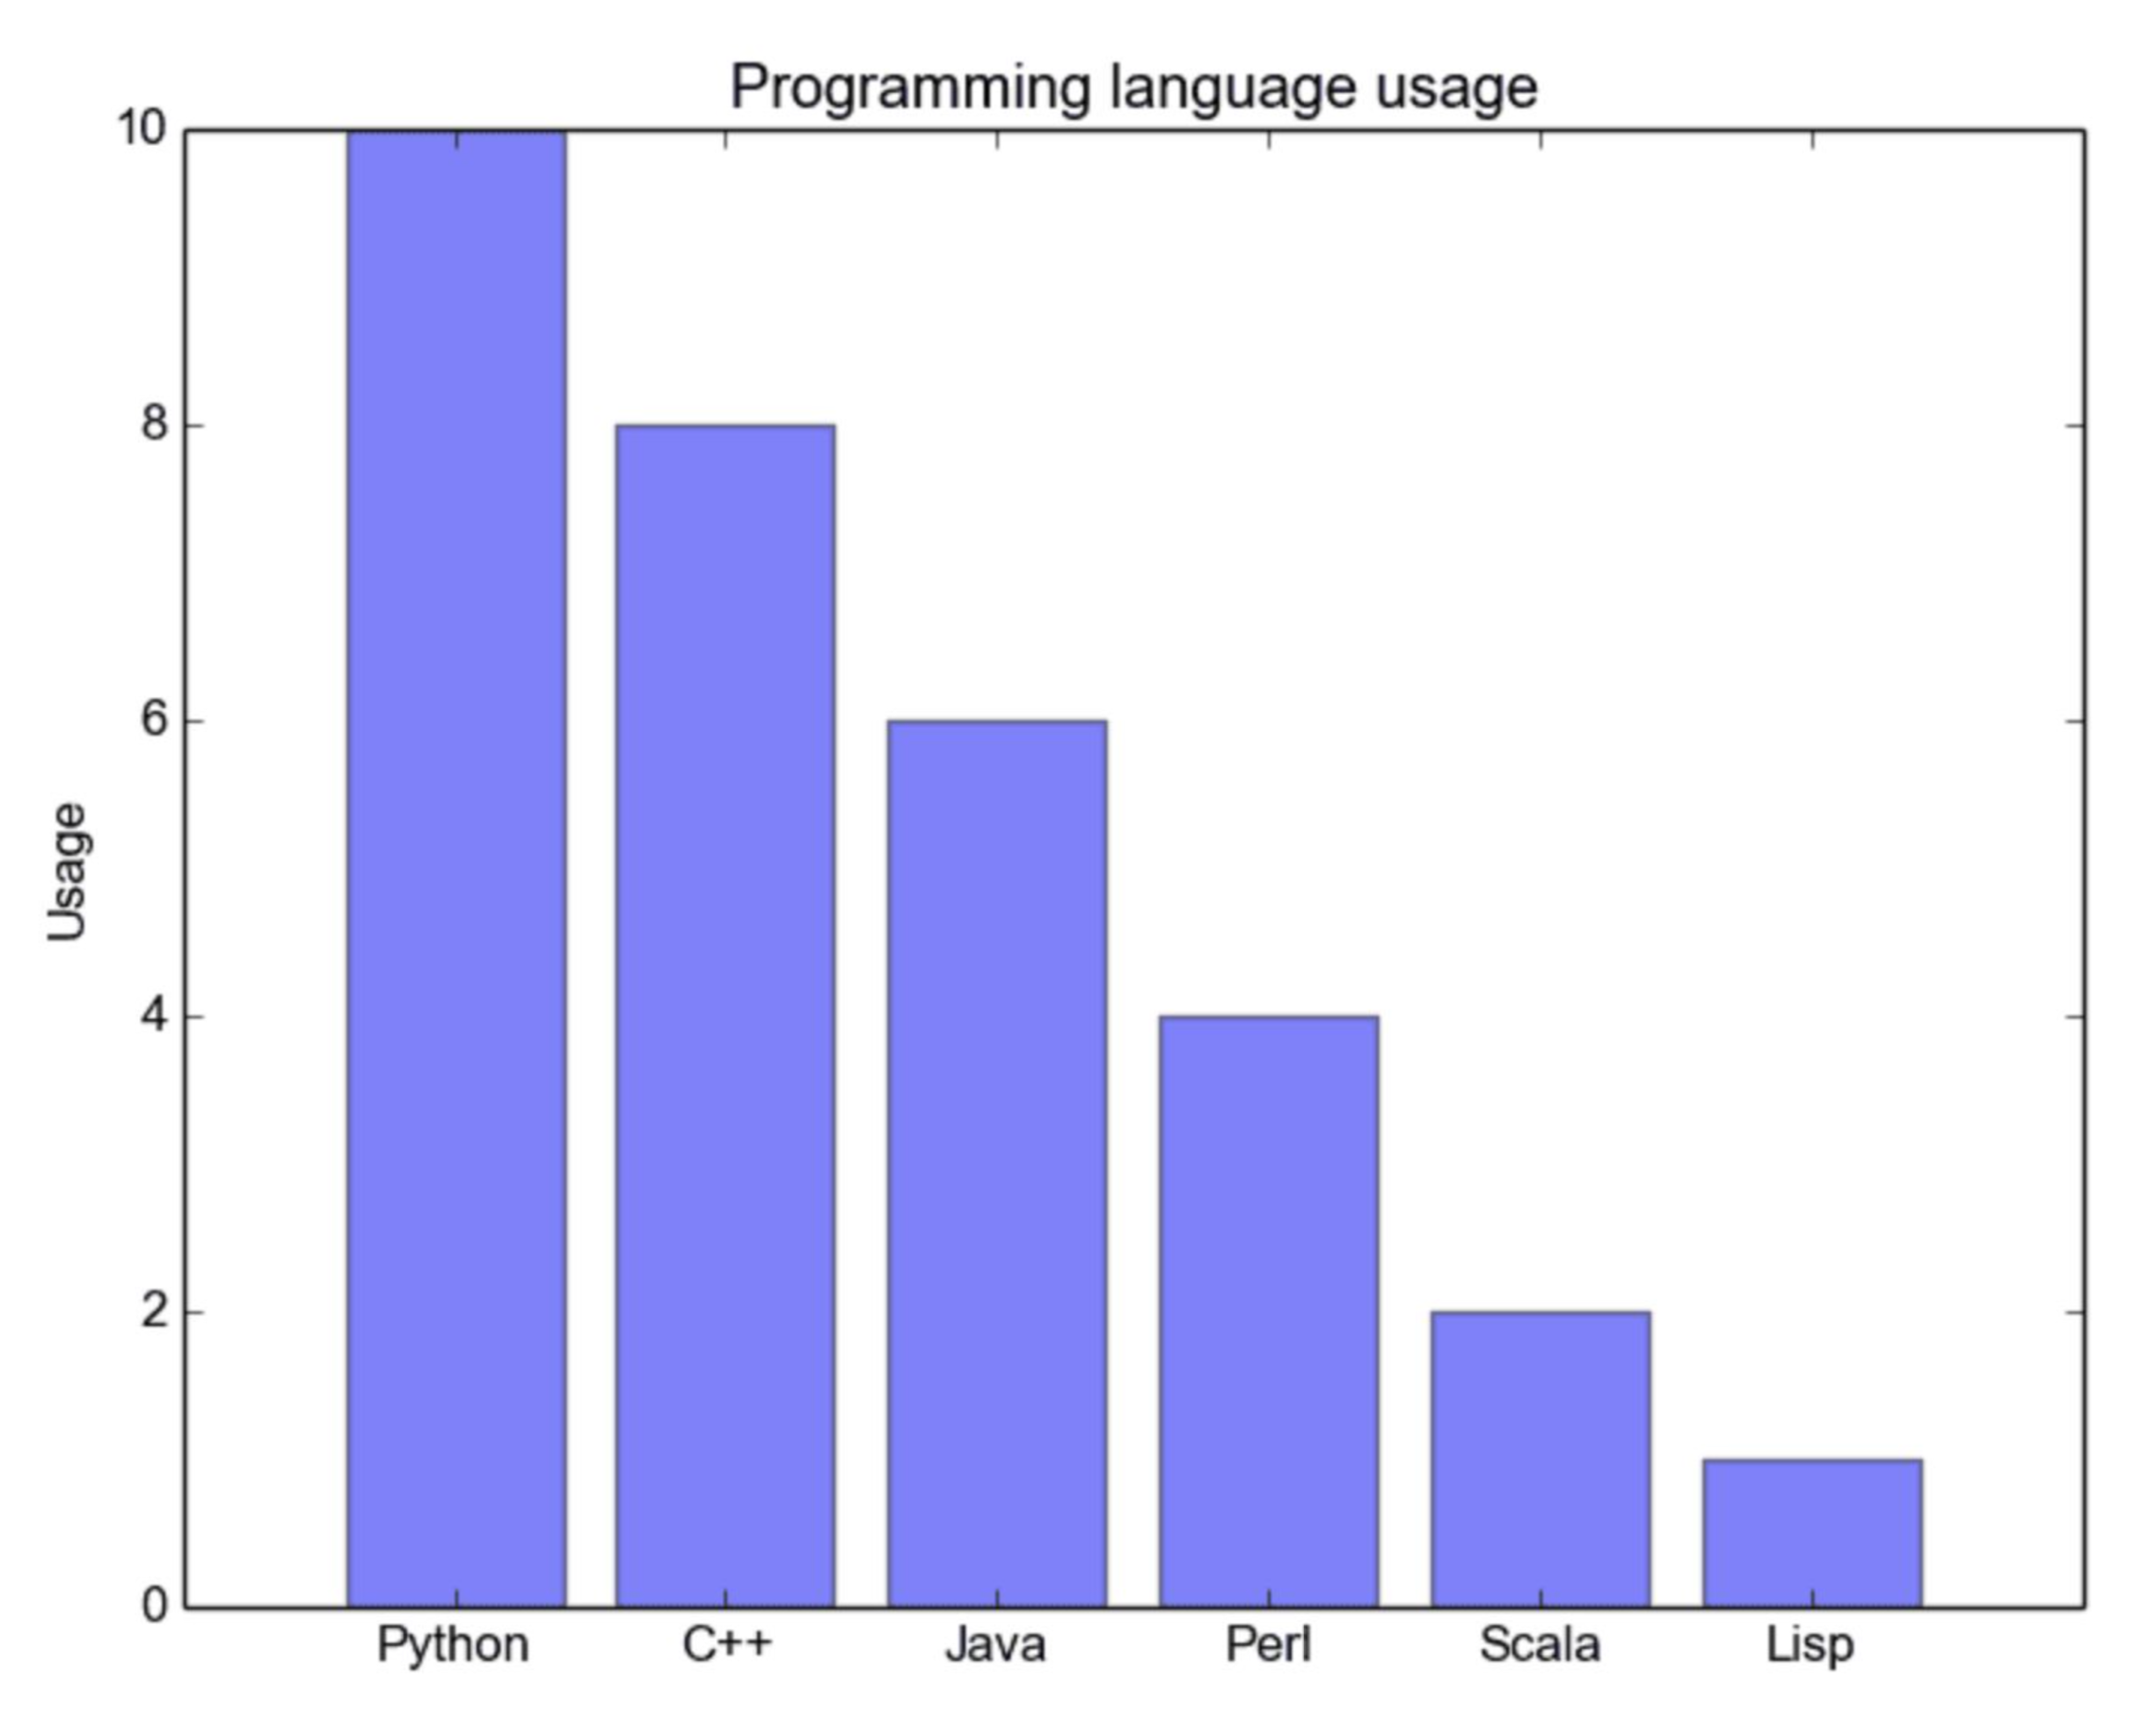
\includegraphics[width=150mm]{images/bar.png}}

\nextexercice
\newpage

% % % % % % % % % % EX03 % % % % % % % % % % % % 


\chapter{Exercise 03:  Scatter Plot}
\exfiles{03\_scatterplot.py}
\turnindir{matplotlib}
\extitle{Scatter Plot}
\extopics{plotting}
\makeheaderfiles

Plot a scatter plot with this data:\\

\begin{lstlisting}
    N = 500
    x = np.random.rand(N)
    y = np.random.rand(N)
    colors = (0,0,0)
    area = np.pi*3
\end{lstlisting}

\centerline{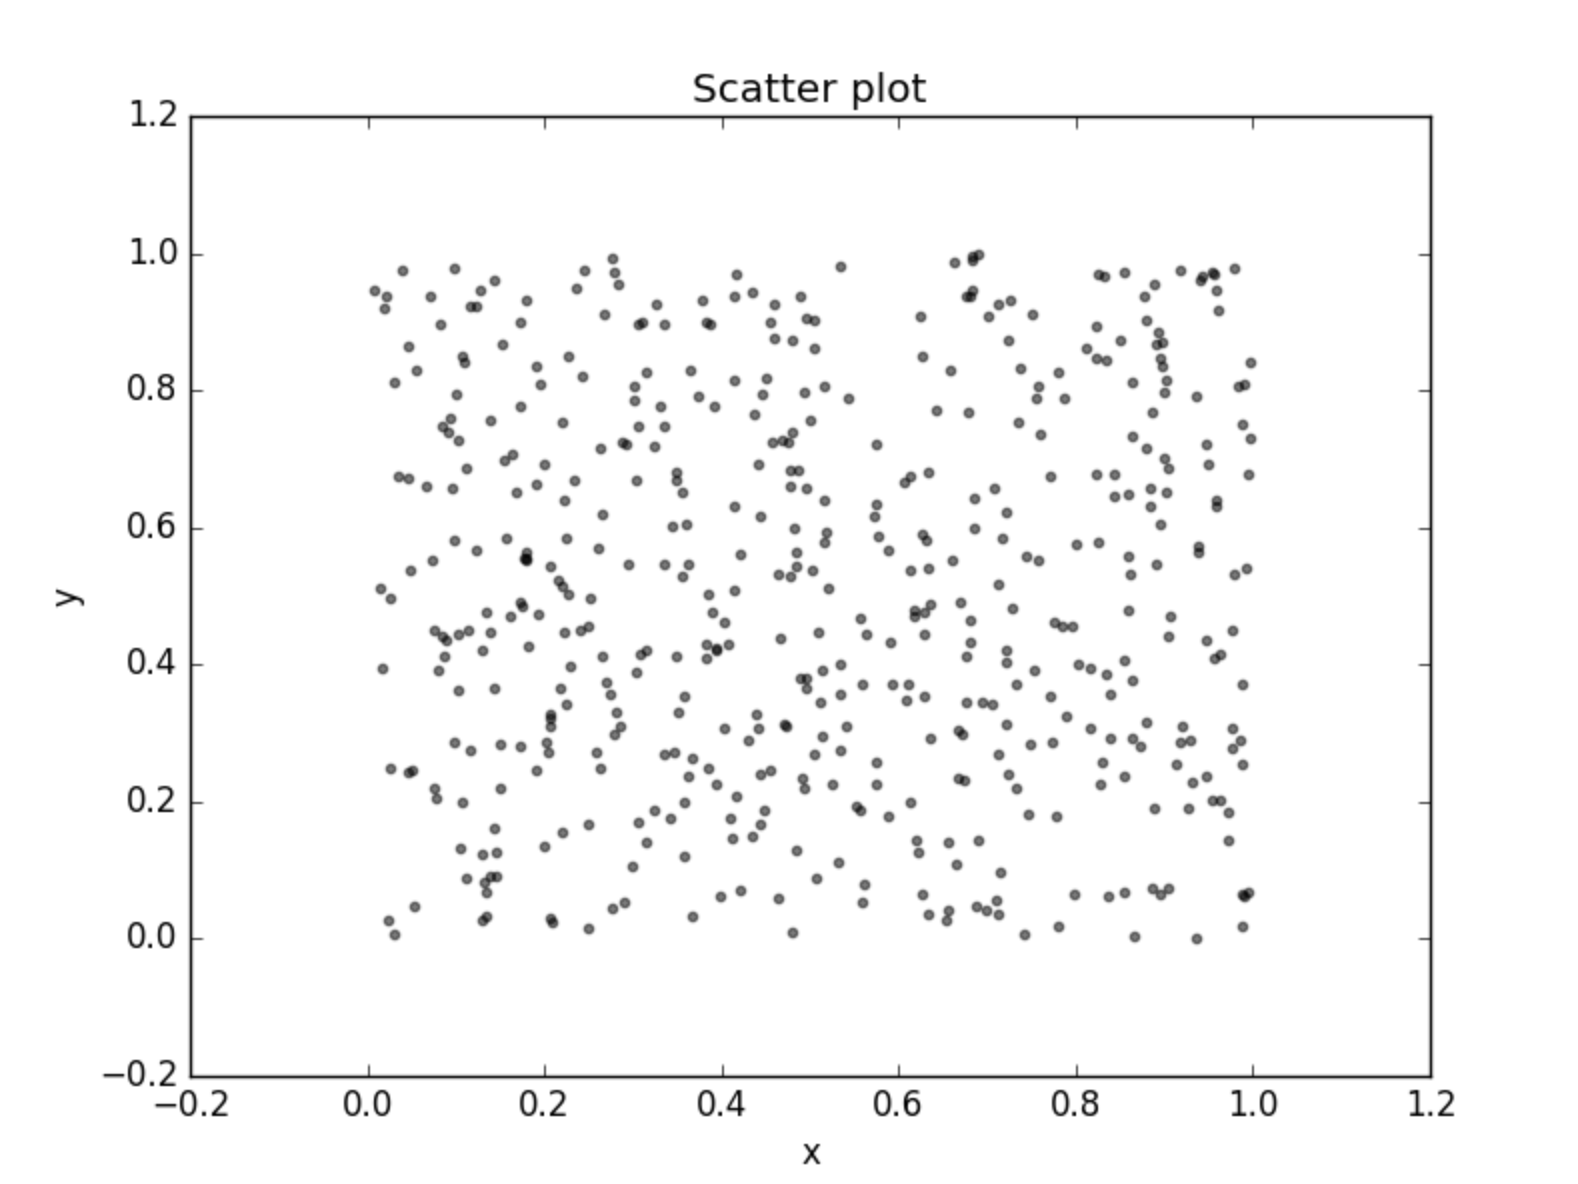
\includegraphics[width=150mm]{images/bw_scatter.png}}

\nextexercice
\newpage

% % % % % % % % % % EX04 % % % % % % % % % % % % 


\chapter{Exercise 04:  Scatter plot with groups}
\exfiles{04\_group\_scatterplot.py}
\turnindir{matplotlib}
\extitle{Scatter plot with groups}
\extopics{plotting}
\makeheaderfiles

Plot a scatter plot with this data:\\

\begin{lstlisting}
    # Create data
    N = 60
    g1 = (0.6 + 0.6 * np.random.rand(N), np.random.rand(N))
    g2 = (0.4+0.3 * np.random.rand(N), 0.5*np.random.rand(N))
    g3 = (0.3*np.random.rand(N),0.3*np.random.rand(N))

    data = (g1, g2, g3)
    colors = ("red", "green", "blue")
    groups = ("coffee", "tea", "water")
\end{lstlisting}

\centerline{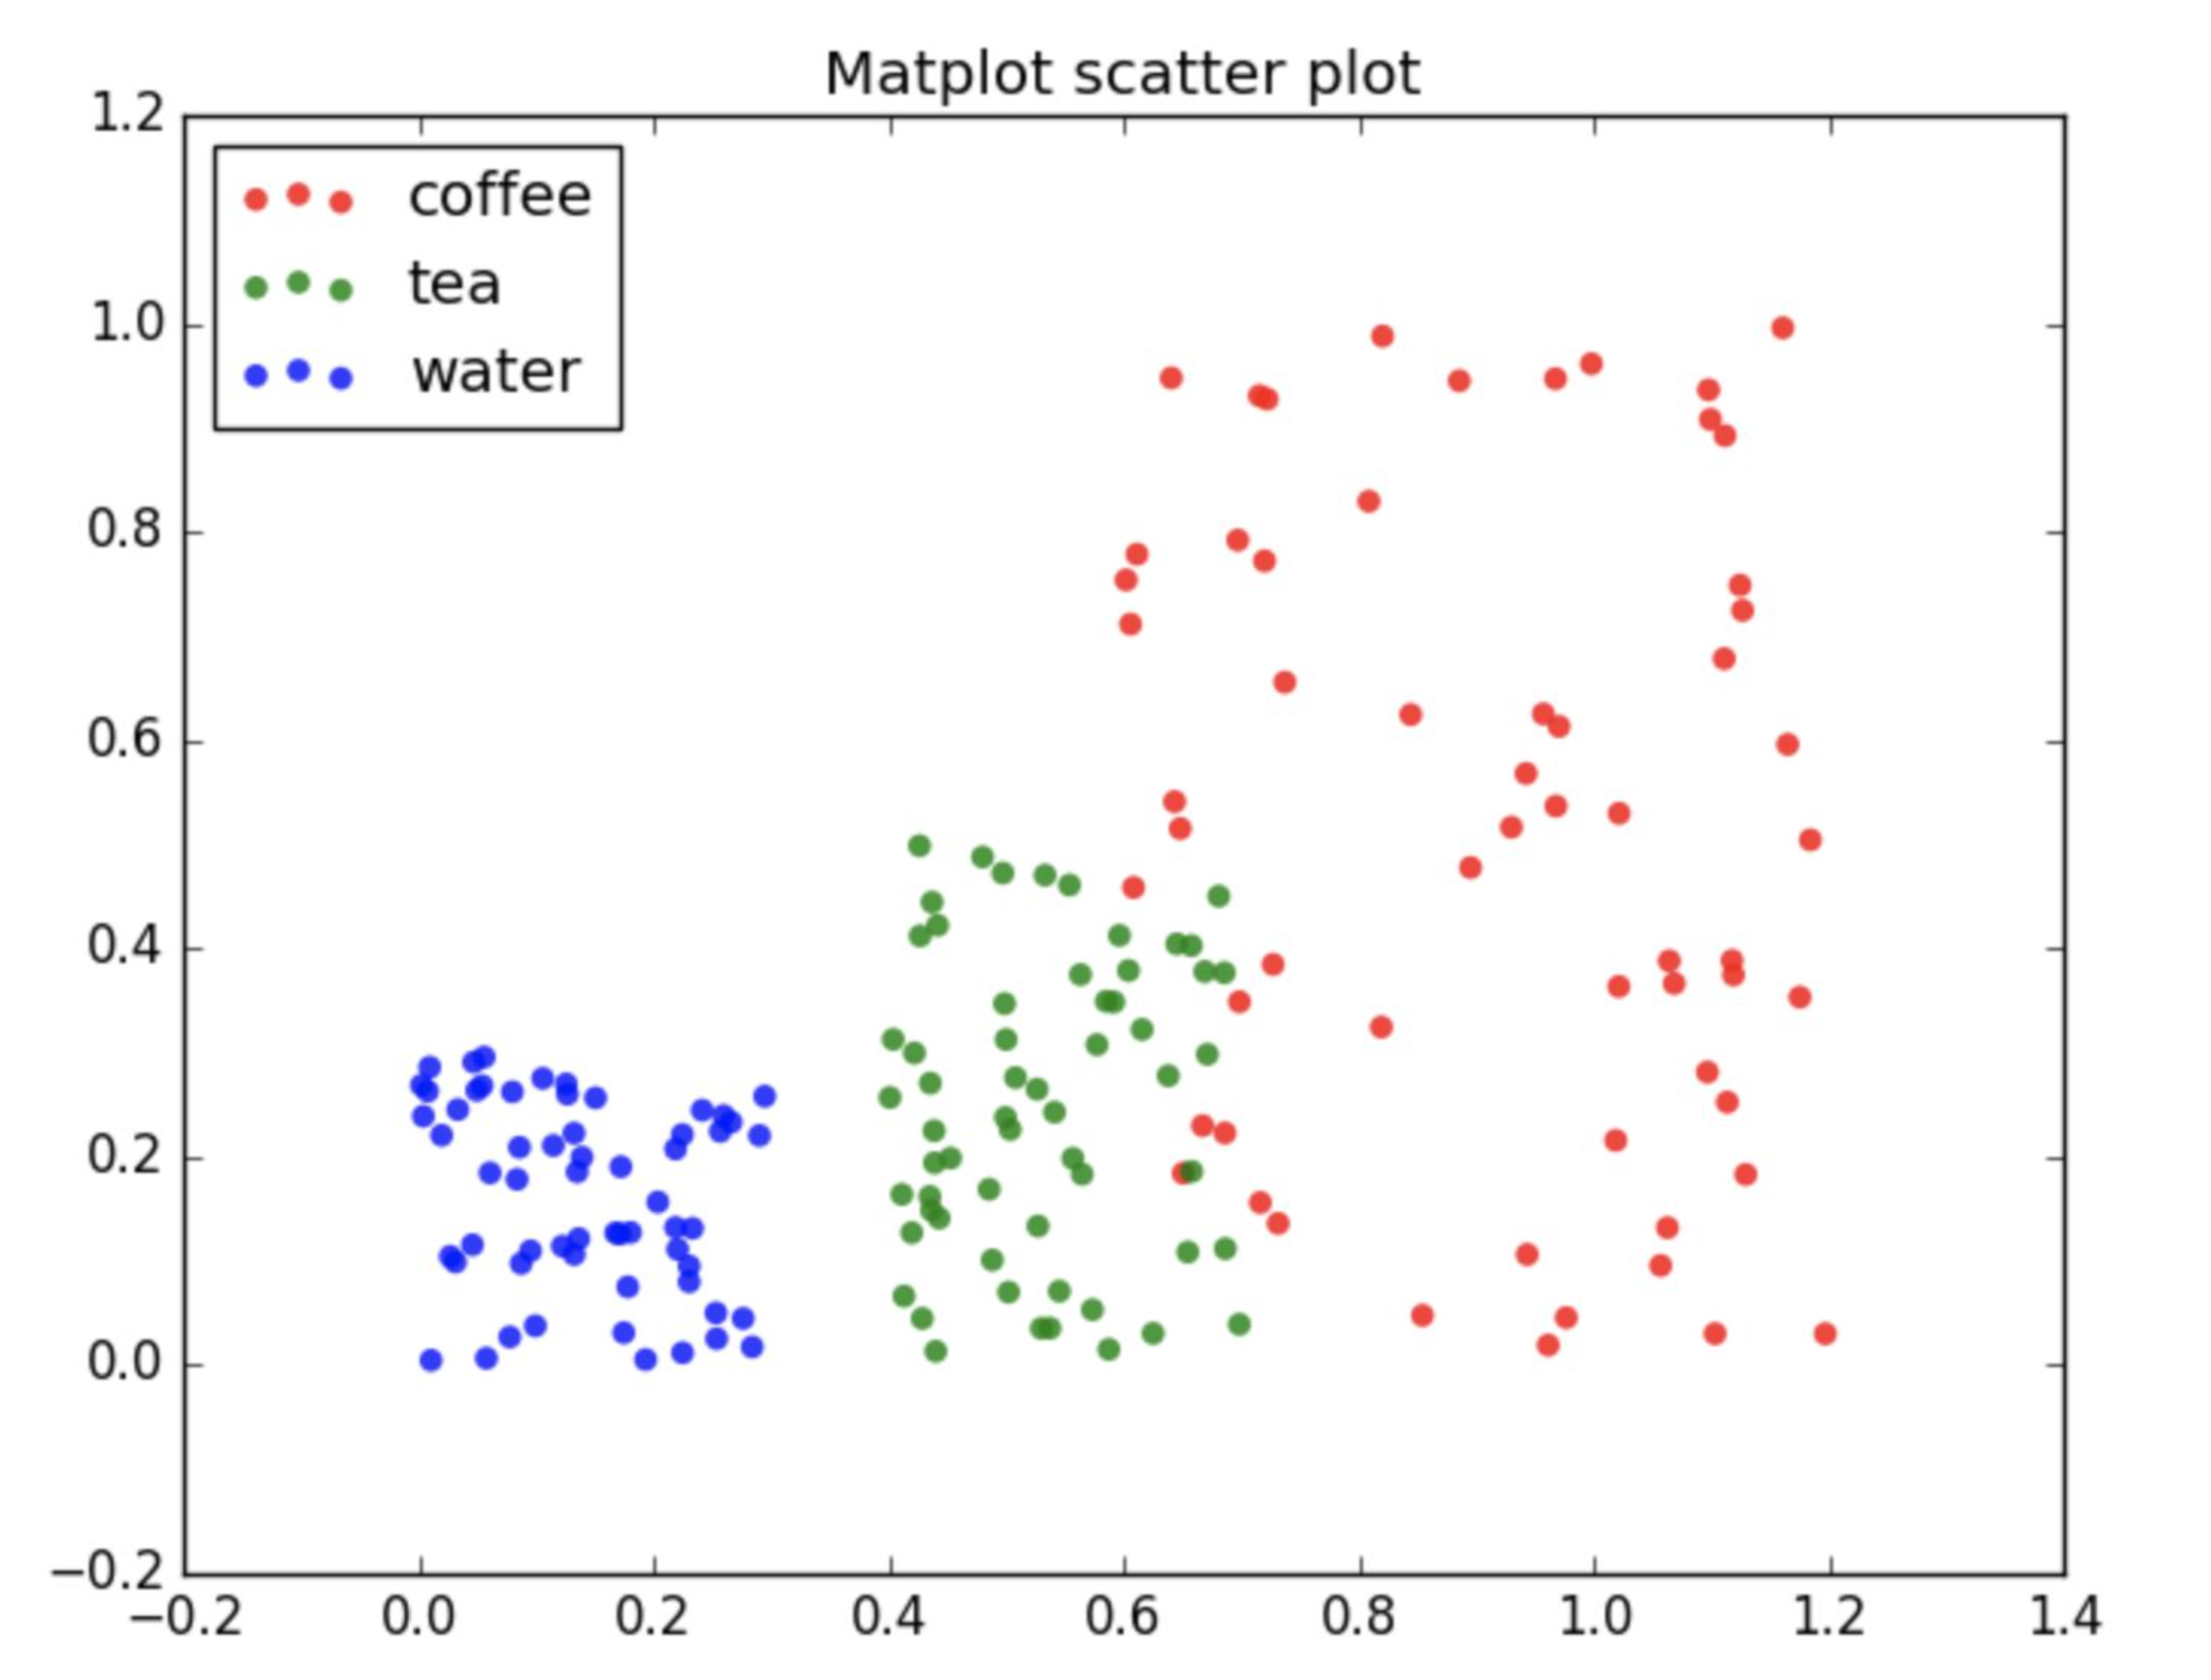
\includegraphics[width=150mm]{images/color_scatter.png}}


\end{document}